\documentclass[border=6pt]{standalone}
\usepackage{tikz}
\usetikzlibrary{arrows.meta, positioning, shapes.geometric, fit, backgrounds, calc, decorations.pathreplacing}

% ═══════════════════════════════════════════════════
% 标准色板 (from tikz-paper-figure-standard.md §1)
% ═══════════════════════════════════════════════════

\definecolor{procFill}{RGB}{219,234,254}
\definecolor{procStroke}{RGB}{37,99,235}
\definecolor{procText}{RGB}{30,58,138}

\definecolor{deciFill}{RGB}{254,243,199}
\definecolor{deciStroke}{RGB}{217,119,6}
\definecolor{deciText}{RGB}{120,53,15}

\definecolor{docFill}{RGB}{224,231,255}
\definecolor{docStroke}{RGB}{79,70,229}
\definecolor{docText}{RGB}{49,46,129}

\definecolor{prepFill}{RGB}{252,231,243}
\definecolor{prepStroke}{RGB}{219,39,119}
\definecolor{prepText}{RGB}{131,24,67}

\definecolor{dbFill}{RGB}{204,251,241}
\definecolor{dbStroke}{RGB}{13,148,136}
\definecolor{dbText}{RGB}{19,78,74}

\definecolor{subFill}{RGB}{255,237,213}
\definecolor{subStroke}{RGB}{234,88,12}
\definecolor{subText}{RGB}{124,45,18}

\definecolor{aiFill}{RGB}{209,250,229}
\definecolor{aiStroke}{RGB}{5,150,105}
\definecolor{aiText}{RGB}{6,78,59}

\definecolor{edgePrimary}{RGB}{17,24,39}
\definecolor{edgePass}{RGB}{22,163,74}
\definecolor{edgeFail}{RGB}{220,38,38}
\definecolor{edgeFeedback}{RGB}{124,58,237}

\begin{document}
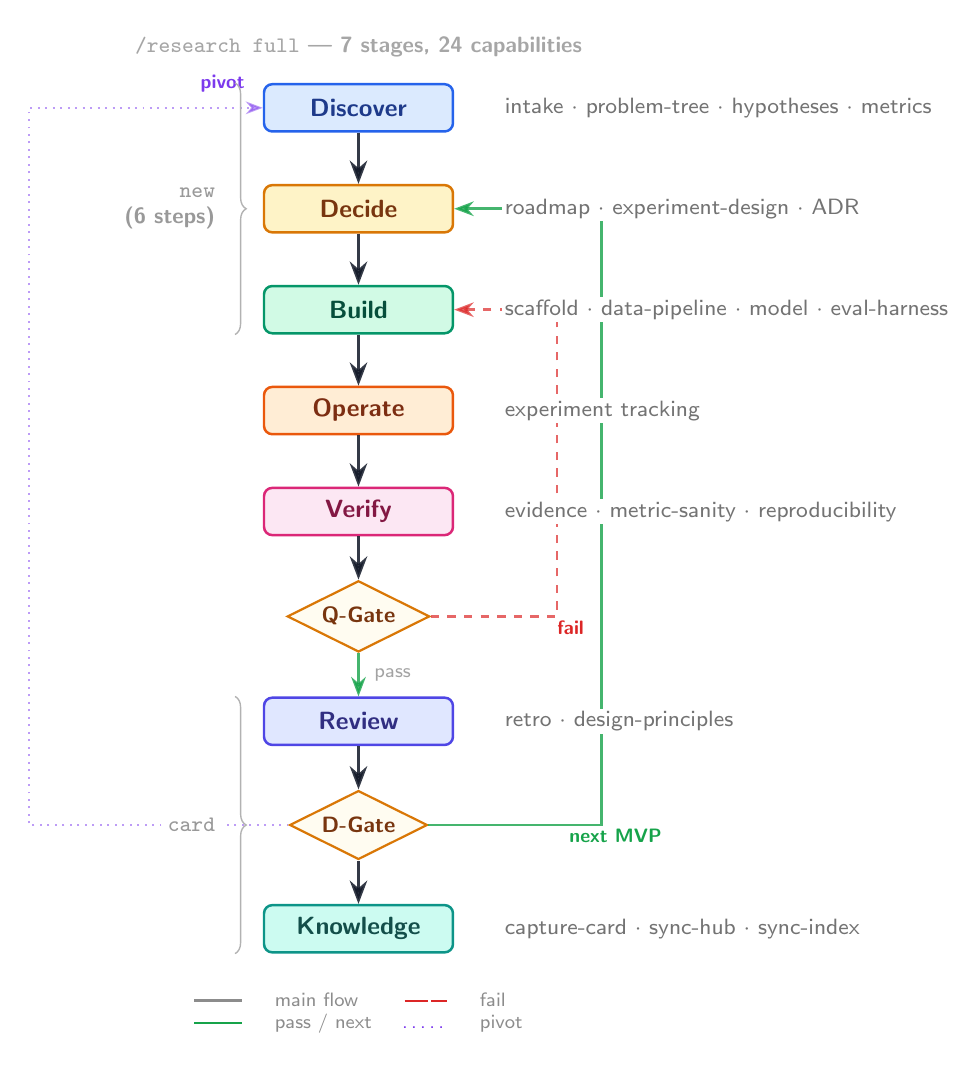
\begin{tikzpicture}[
    >=Stealth,
    node distance=0.65cm and 1.2cm,
    every node/.style={font=\sffamily},
    % ═══════════ Node styles ═══════════
    stage/.style={
        rounded corners=3pt, line width=0.9pt,
        minimum width=2.4cm, minimum height=0.6cm,
        inner sep=4pt, align=center, font=\sffamily\small\bfseries
    },
    gate/.style={
        diamond, line width=0.8pt, aspect=2.0,
        inner sep=2pt, align=center, font=\sffamily\footnotesize\bfseries,
        draw=deciStroke, fill=deciFill!25, text=deciText
    },
    capbox/.style={
        font=\sffamily\footnotesize, text=black!55, align=left,
        fill=white, inner sep=1pt
    },
    annot/.style={font=\sffamily\scriptsize, text=black!45},
    feedlbl/.style={font=\sffamily\scriptsize\bfseries},
    % ═══════════ Edge styles ═══════════
    primary/.style={->, edgePrimary, line width=1.2pt, opacity=0.85},
    gatepass/.style={->, edgePass, line width=0.9pt, opacity=0.80},
    gatefail/.style={->, edgeFail, line width=0.9pt, opacity=0.70, dashed},
    feedback/.style={->, edgeFeedback, line width=0.7pt, opacity=0.50, dotted},
]

% ═══════════════════════════════════════════════════
% Main vertical column (top → bottom)
% ═══════════════════════════════════════════════════

% --- Stage nodes (positioned first, annotations drawn later) ---
\node[stage, draw=procStroke, fill=procFill, text=procText]
    (discover) {Discover};
\node[stage, draw=deciStroke, fill=deciFill, text=deciText,
    below=0.65cm of discover]
    (decide) {Decide};
\node[stage, draw=aiStroke, fill=aiFill, text=aiText,
    below=0.65cm of decide]
    (build) {Build};
\node[stage, draw=subStroke, fill=subFill, text=subText,
    below=0.65cm of build]
    (operate) {Operate};
\node[stage, draw=prepStroke, fill=prepFill, text=prepText,
    below=0.65cm of operate]
    (verify) {Verify};
\node[gate, below=0.55cm of verify]
    (qgate) {Q-Gate};
\node[stage, draw=docStroke, fill=docFill, text=docText,
    below=0.55cm of qgate]
    (review) {Review};
\node[gate, below=0.55cm of review]
    (dgate) {D-Gate};
\node[stage, draw=dbStroke, fill=dbFill, text=dbText,
    below=0.55cm of dgate]
    (knowledge) {Knowledge};

% ═══════════════════════════════════════════════════
% Main flow arrows (vertical, no crossing)
% ═══════════════════════════════════════════════════

\draw[primary] (discover) -- (decide);
\draw[primary] (decide) -- (build);
\draw[primary] (build) -- (operate);
\draw[primary] (operate) -- (verify);
\draw[primary] (verify) -- (qgate);
\draw[gatepass] (qgate) -- (review) node[annot, midway, right, xshift=2pt] {pass};
\draw[primary] (review) -- (dgate);
\draw[primary] (dgate) -- (knowledge);

% ═══════════════════════════════════════════════════
% Feedback arrows — dedicated SIDE CHANNELS (no crossing)
% ═══════════════════════════════════════════════════

% Margin x-coordinates (well outside main column)
\pgfmathsetmacro{\rightchannel}{2.8}   % right margin for fail + next MVP
\pgfmathsetmacro{\leftchannel}{-4.5}   % left margin for pivot (wide: clears brace labels)

% --- Q-Gate FAIL → Build (RIGHT channel) ---
\draw[gatefail]
    (qgate.east) -- ++(\rightchannel - 1.2, 0)
    coordinate (failR)
    -- (failR |- build.east)
    -- (build.east);
\node[feedlbl, text=edgeFail] at ([xshift=5pt, yshift=-4pt]failR) {fail};

% --- D-Gate "next MVP" → Decide (RIGHT channel, offset further right) ---
\draw[gatepass]
    (dgate.east) -- ++(\rightchannel - 0.6, 0)
    coordinate (nextR)
    -- (nextR |- decide.east)
    -- (decide.east);
\node[feedlbl, text=edgePass] at ([xshift=5pt, yshift=-4pt]nextR) {next MVP};

% --- D-Gate "pivot" → Discover (LEFT channel) ---
\draw[feedback]
    (dgate.west) -- ++(\leftchannel + 1.2, 0)
    coordinate (pivotL)
    -- (pivotL |- discover.west)
    -- (discover.west);
% pivot label near Discover (far from "card" label near D-Gate)
\node[feedlbl, text=edgeFeedback, anchor=south east]
    at ([xshift=-3pt, yshift=2pt]discover.west) {pivot};

% ═══════════════════════════════════════════════════
% Capability annotations (drawn AFTER arrows so fill=white covers crossings)
% ═══════════════════════════════════════════════════

\node[capbox, right=0.6cm of discover]
    {intake $\cdot$ problem-tree $\cdot$ hypotheses $\cdot$ metrics};
\node[capbox, right=0.6cm of decide]
    {roadmap $\cdot$ experiment-design $\cdot$ ADR};
\node[capbox, right=0.6cm of build]
    {scaffold $\cdot$ data-pipeline $\cdot$ model $\cdot$ eval-harness};
\node[capbox, right=0.6cm of operate]
    {experiment tracking};
\node[capbox, right=0.6cm of verify]
    {evidence $\cdot$ metric-sanity $\cdot$ reproducibility};
\node[capbox, right=0.6cm of review]
    {retro $\cdot$ design-principles};
\node[capbox, right=0.6cm of knowledge]
    {capture-card $\cdot$ sync-hub $\cdot$ sync-index};

% ═══════════════════════════════════════════════════
% Sub-command labels (braces on LEFT margin)
% ═══════════════════════════════════════════════════

% "/research new" bracket: Discover → Build (first 6 steps)
\draw[decorate, decoration={brace, amplitude=4pt},
    black!30, line width=0.5pt]
    ([xshift=-10pt]discover.north west) -- ([xshift=-10pt]build.south west)
    node[midway, left=5pt, font=\sffamily\footnotesize\bfseries, text=black!40,
         align=right, fill=white, inner sep=2pt]
    {\texttt{new}\\(6 steps)};

% "/research card" bracket: Review → Knowledge
\draw[decorate, decoration={brace, amplitude=4pt},
    black!30, line width=0.5pt]
    ([xshift=-10pt]review.north west) -- ([xshift=-10pt]knowledge.south west)
    node[midway, left=5pt, font=\sffamily\footnotesize\bfseries, text=black!40,
         align=right, fill=white, inner sep=2pt]
    {\texttt{card}};

% "/research full" label at top
\node[annot, font=\sffamily\footnotesize\bfseries, text=black!35,
    above=6pt of discover]
    {\texttt{/research full} --- 7 stages, 24 capabilities};

% ═══════════════════════════════════════════════════
% Legend (bottom, outside main content)
% ═══════════════════════════════════════════════════

\node[annot, anchor=north, font=\sffamily\scriptsize]
    at ([yshift=-10pt]knowledge.south) (leg) {%
    \begin{tabular}{@{}rl@{\hspace{10pt}}rl@{}}
    \rule[0.5ex]{0.6cm}{1.2pt} & main flow &
    {\color{edgeFail}\rule[0.5ex]{0.3cm}{0.9pt}\hspace{1pt}\rule[0.5ex]{0.2cm}{0.9pt}} & fail \\
    {\color{edgePass}\rule[0.5ex]{0.6cm}{0.9pt}} & pass / next &
    {\color{edgeFeedback}\hbox to 0.6cm{\dotfill}} & pivot \\
    \end{tabular}%
};

\end{tikzpicture}
\end{document}
